\section{Evaluation}\seclabel{Evaluation}


\subsection{\WatProvenance{} Specifications}
\subsection{A Case Study}

\subsection{Shim Overheads}
We now measure the performance overheads of \fluent{} shims. \fluent{} shims
increase the latency and reduce throughput of black boxes for two reasons.
First, there is a latency overhead in proxying messages to and from a black
box. Second, there is a latency overhead in persisting the messages to a
relational database.  Some of these overheads can be avoided---e.g., \fluent{}
shims buffer messages in memory and only periodically persist them to a
relation database---but some overhead is unavoidable.

In this subsection, we measure the overheads introduced by \fluent{} shims for
two black boxes: Redis and Amazon S3. We do so with the following three step
experiment.
\begin{enumerate}
  \item
    We measure the throughput of each black box when it is not wrapped in a
    \fluent{} shim.
  \item
    We measure the throughput of each black box when it is wrapped with a
    \fluent{} shim that does not persist any messages. This ``partial shim''
    incurs the overheads of proxying messages but not the overheads of
    persisting them.
  \item
    We measure the throughput of each black box when it is wrapped with a fully
    functional \fluent{} shim that periodically persists messages to a
    relational database. Unlike the partial shim, This ``full shim'' incurs all
    of the overheads of a \fluent{} shim.
\end{enumerate}

To measure the throughput of Redis, we have a single client perform small two
byte set requests to a single key for five seconds. To measure the throughput
of S3, we have a single client create, read, and delete 25 objects in a single
bucket. Each object is 1 KB. We run clients, shims, and black boxes on
t2.xlarge instances on Amazon EC2. We colocate shims with their black boxes,
but otherwise place clients and black boxes on different instances within the
same availability zone. We repeat each throughput measurement twenty times.
Box plots of these throughput measurements are shown in \figref{Shims}.

\begin{figure}[ht]
  \centering
  \begin{subfigure}[b]{\columnwidth}
    \centering
    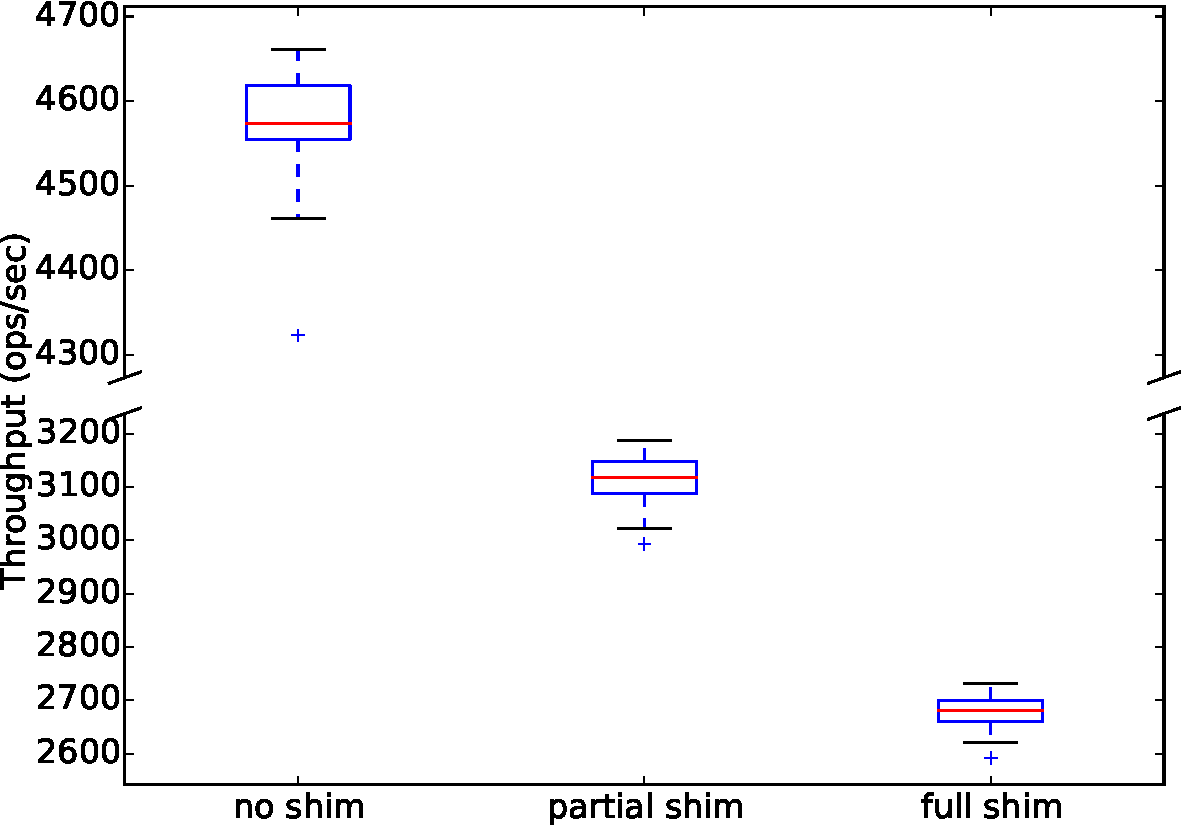
\includegraphics[width=0.8\columnwidth]{figures/redis_shim.pdf}
    \caption{Redis throughput}
    \figlabel{RedisShim}
  \end{subfigure}

  \begin{subfigure}[b]{\columnwidth}
    \centering
    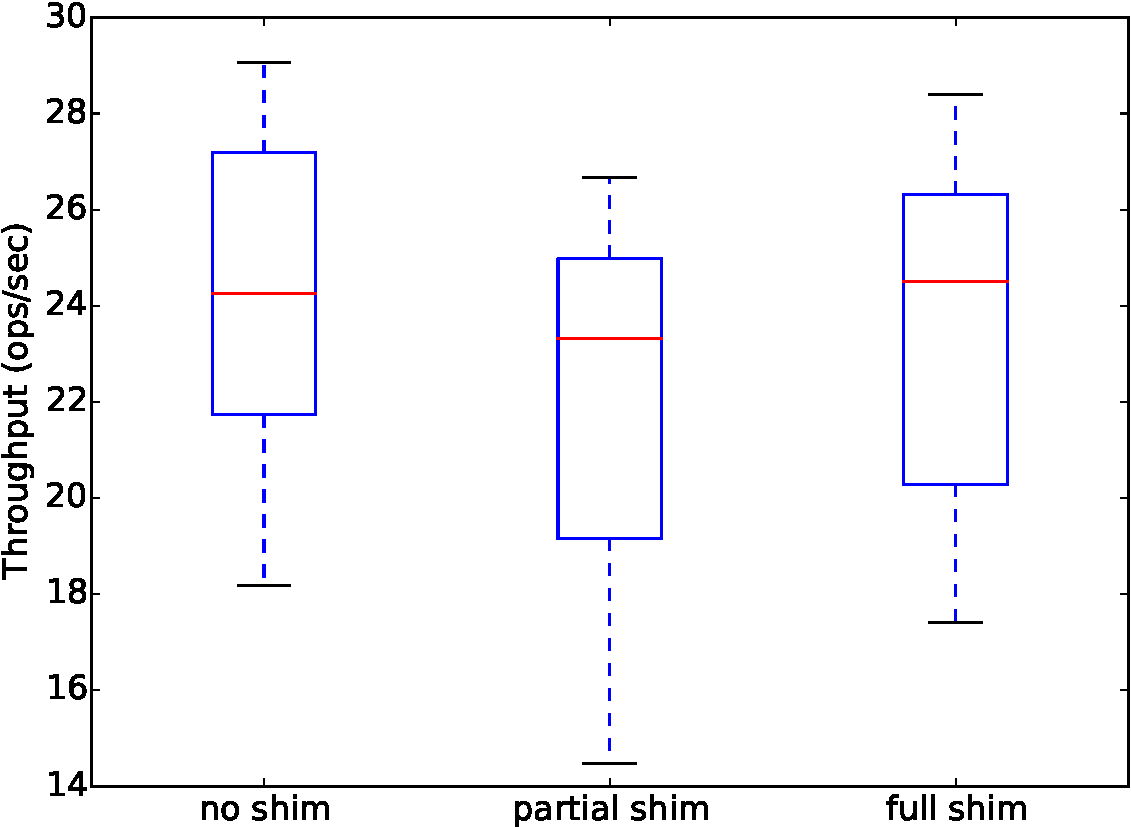
\includegraphics[width=0.8\columnwidth]{figures/s3_shim.pdf}
    \caption{S3 throughput}
    \figlabel{S3Shim}
  \end{subfigure}%
  \caption{The overheads of \fluent{} shims}
  \figlabel{Shims}
\end{figure}

% (4566.224999999999  , 332.309657849422)
% (3111.4139999999998 , 225.28554831590938)
% (2676.5609999999997 , 144.54921507915557)
Redis averages a throughput of 4566 set requests per second (with standard
deviation 322) when not wrapped with a \fluent{} shim. When it is wrapped with
a \fluent{} shim that does not persist messages, the throughput drops to an
average of 3111 set requests per second (with a standard deviation of 225).
When Redis is wrapped with a fully functional shim, its throughput drops to
2676 set request per second. These large decreases in throughput are expected.
Redis is a lightweight system, and the time it takes to service a single set
request is very low. Thus, even small overheads can significantly decrease
throughput.  While these overheads are fundamental to our shim-based approach,
they will likely decrease as we continue to optimize \fluent{}'s prototype
implementation.

% (24.222414999999998 , 14.674786717547207)
% (22.34917           , 15.440412655172143)
% (23.572789999999998 , 15.308642281338997)
Unlike Redis, S3's throughput is relatively unaffected by the overheads of the
shims. Without any shim, S3 averages a throughput of 24.22 operations per
second (with standard deviation 14.67). This throughput drops only slightly to
22.35 operations per second (with standard deviation 15.44) and 23.58
operations per second (with standard deviation 15.31) when S3 is wrapped with a
partial and full\fluent{} shim respectively. In contrast to Redis, S3
sacrifices low latency and high throughput for availability. Thus, the small
overheads introduced by the shims are largely negligible.
